\chapter{Programmazione aggregata}\label{ch:aggregate}

La crescita esponenziale di dispositivi informatici di varia natura inseriti in contesti quotidiani ha avuto un impatto globale notevole.
Questo insieme di entità connesse (\Cref{fig:iot}) ha dato luogo a ciò che viene definito \emph{Internet of Things} (\emph{IoT})~\cite{ashton2009internet}:
sistemi costituiti da reti di oggetti fisici, tipicamente embedded, che interagiscono mediante la rete Internet.

\begin{figure}[htbp]
  \centering
  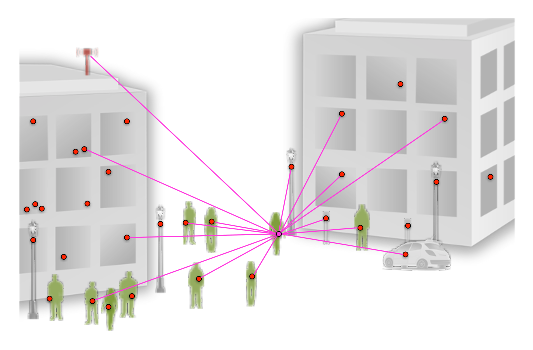
\includegraphics[width=0.8\textwidth]{res/fig/iot.eps}%
  \caption[
    Possibile scenario di rete in contesto urbano.
  ]{
    Possibile scenario di rete in contesto urbano.

    \nameCref{fig:iot} ripresa da~\cite{7274429}.
  }%
  \label{fig:iot}
\end{figure}

L'approccio tradizionale per la realizzazione di sistemi in questo contesto è sempre stato dal punto di vista del singolo dispositivo,
il quale è preso come unità fondamentale, connessa con il mondo fisico e con gli altri device.
In questo punto di vista, l'insieme di tutti i comportamenti individuali delle unità determina il funzionamento del sistema.
Tale approccio, per quanto valido, può risultare limitante in sistemi distribuiti eterogenei, nei quali possono presentarsi diversi problemi legati all'organizzazione della rete
e alla sua gestione a causa delle dimensioni e delle differenze tra i dispositivi.
Tali problematiche, generalmente, vorrebbero essere gestite ad un livello di astrazione più elevato.

L'\emph{aggregate programming}, o \emph{programmazione aggregata}, costituisce un'alternativa all'approccio ``classico''
volta a semplificare la progettazione, creazione e manutenzione di sistemi distribuiti complessi.
La programmazione aggregata, infatti, ragiona su larga scala, cercando di spostare l'attenzione sul \emph{collettivo di dispositivi} che collaborano,
astraendo dai dettagli relativi al singolo device~\cite{7274429} per quanto possibile.
% a capo rimosso
% TODO: rifai
L'idea alla base è dunque di definire una modalità di deduzione del comportamento locale al singolo dispositivo a partire dal comportamento globale, di più alto livello,
effettuando un \emph{mapping da globale a locale}.
In contesti distribuiti, sono stati individuati principalmente due punti di vista a questo livello di astrazione~\cite{aggregatescala-pmldc2016}: locale o globale.
Il primo, detto anche \emph{device-centric} (\Cref{fig:device-centric}), fa riferimento alla computazione aggregata eseguita dal singolo dispositivo.
Questo può essere considerato il punto di vista tradizionale.

\begin{figure}[htbp]
  \centering
  % \includesvg[width=.5\textwidth]{res/fig/device-centric.svg}
  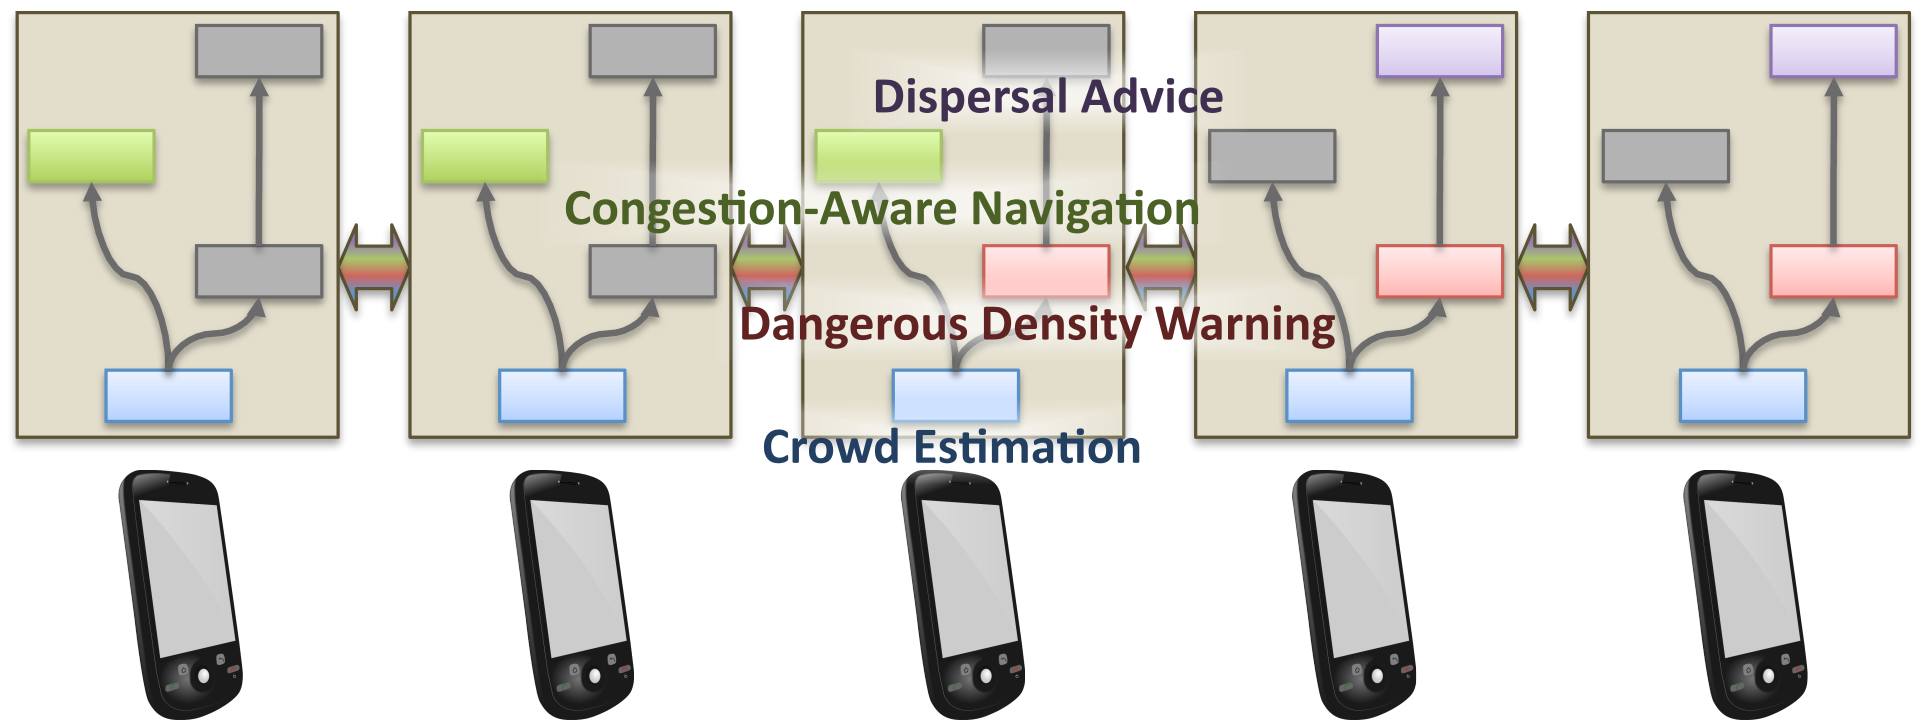
\includegraphics[width=.55\textwidth]{res/fig/device-centric.png}
  \caption{Livello di astrazione \emph{device-centric}}%
  \label{fig:device-centric}
\end{figure}

Il secondo punto di vista, detto \emph{aggregate view} (\Cref{fig:aggregate}), sposta invece l'attenzione sulla computazione svolta dal sistema aggregato come singola unità.
Rispetto all'approccio tradizionale, tale punto di vista sposta maggiormente l'attenzione dal \emph{come} il sistema possa funzionare
al \emph{cosa} effettivamente si desidera che faccia.

\begin{figure}[htbp]
  \centering
  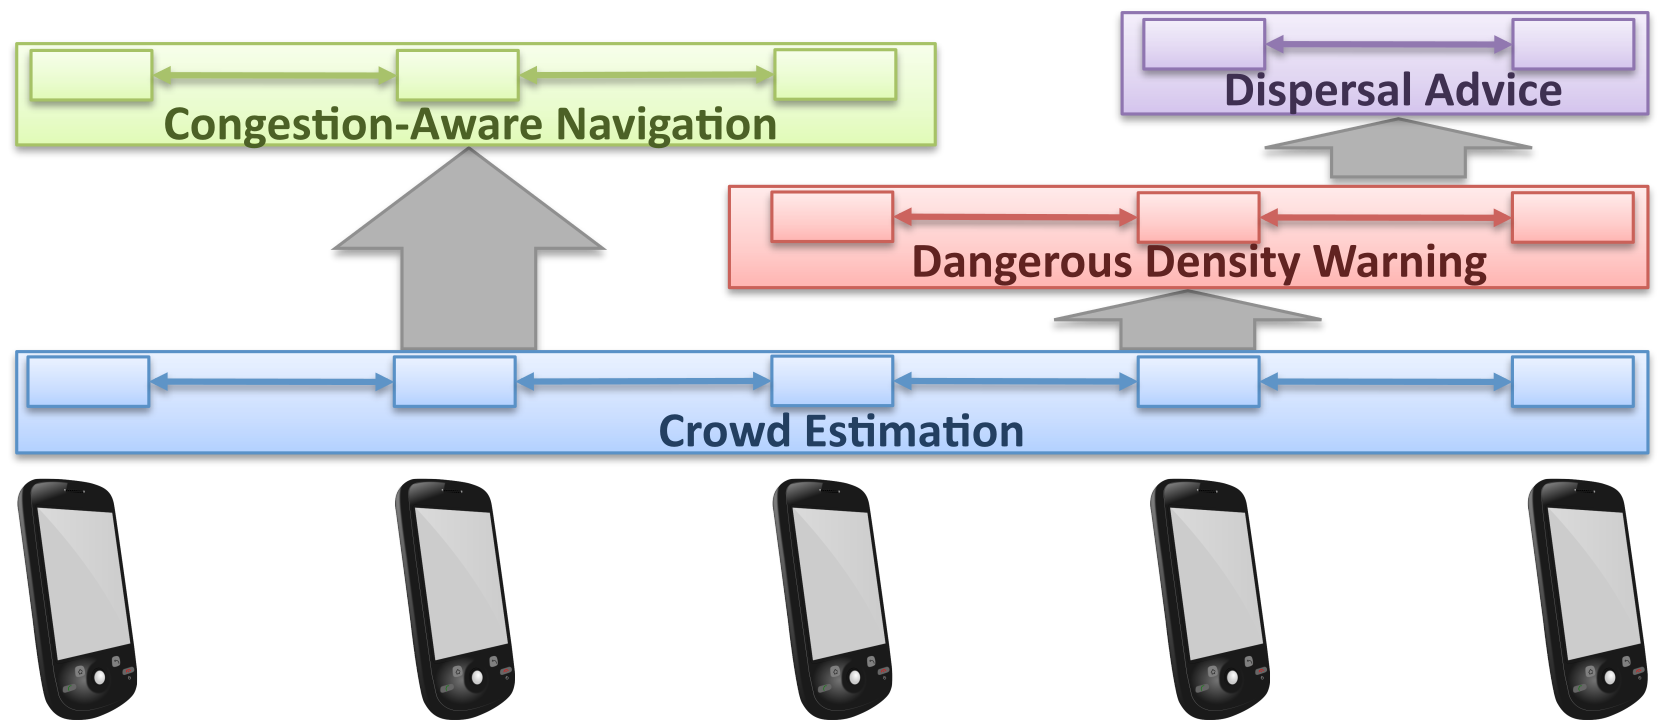
\includegraphics[width=.55\textwidth]{res/fig/aggregate.png}
  % \includesvg[width=.5\textwidth]{res/fig/aggregate.svg}
  \caption{Livello di astrazione \emph{aggregate view}}%
  \label{fig:aggregate}
\end{figure}

In letteratura, sono state adottate diverse strategie~\cite{7274429} ad un livello di astrazione così elevato.
Ad esempio, l'approccio \emph{TOTA} (``\emph{Tuples On The Air}''~\cite{10.1145/1538942.1538945}) prevede di rendere le interazioni tra i dispositivi implicite,
mentre l'\emph{Origami Shape Language}~\cite{nagpal2001programmable} si basa sulla composizione di costruzioni geometriche e topologiche attraverso operazioni di \emph{folding}.
Altri esempi sono le tecniche di sintesi dei dati provenienti da alcune regioni spazio-temporali per inviarli come stream ad altre regioni delineate con \emph{TinyDB}~\cite{1017485}
o le modalità con cui modelli di \emph{computazione cloud} come \emph{MapReduce}~\cite{10.1145/1327452.1327492} dividono la computazione in modo automatico tra i nodi.
Infine, linguaggi come \emph{Protelis}~\cite{PianiniSASOTutorial2017}, di cui tratteremo meglio in~\Cref{sec:protelis}, forniscono costrutti generalizzabili per la computazione spazio-temporale che si prestano ad un uso in ambiente IoT.

Lo studio dei suddetti approcci ha permesso di fare considerazioni sulle modalità di programmazione dei sistemi situati di larga scala;
innanzitutto, laddove non sia richiesto al programmatore di gestire i meccanismi di interazione, le modalità di coordinazione dovrebbero essere robuste e nascoste ``\emph{under the hood}''~\cite{7274429}.
Poi, il framework di programmazione dovrebbe essere modulare, e tali moduli dovrebbero essere componibili in modo semplice e trasparente.
Infine, deve essere possibile fornire meccanismi di coordinazione differenti per diverse parti del sistema aventi regioni dello spazio e tempi distinti.

La programmazione aggregata cerca di rispondere alle seguenti esigenze~\cite{7274429}:

% TODO: collassa elenco puntato
\begin{itemize}
  \item la ``macchina'' programmata non è il singolo dispositivo, bensì il loro agglomerato; % a \emph{regione} dell'ambiente computazionale che astrae dai dettagli specifici
  \item il ``programma'' è specificato come manipolazione di strutture dati distribuite che evolvono nel tempo dette \emph{computational fields};
  % TODO: modularità e componibilità
  \item tali manipolazioni vengono eseguite dai dispositivi inseriti all'interno della regione, tramite l'uso di meccanismi di coordinazione resilienti e di interazioni basate sulla prossimità.
\end{itemize}

In questo modo, i meccanismi di coordinazione, spesso complessi, vengono nascosti facilitando la costruzione e favorendo la modularità.
In particolare, il paradigma si struttura su più livelli di astrazione, come è possibile vedere in~\Cref{fig:stack}.

Nelle \nameCrefs{sec:field-calculus} successive analizzeremo più nel dettaglio alcuni di questi.

\begin{figure}[htbp]
  \centering
  \includesvg[width=0.55\textwidth]{res/fig/stack-2.svg}%
  \caption[
    Principali livelli dell'\emph{Aggregate Programming}.
  ]{
    Principali livelli dell'\emph{Aggregate Programming}.

    \nameCref{fig:stack} ripresa da~\cite{ProtelisSAC14}.
  }%
  \label{fig:stack}
\end{figure}

\section{Field calculus e Building Blocks}\label{sec:field-calculus}

Al livello più basso della struttura rappresentata in \Cref{fig:stack} si trova il \emph{field calculus}~\cite{tocl}.
Esso è un \emph{core calculus}, ovvero un modello teorico di programmazione che riassume la semantica operazionale minimale necessaria alla progettazione di un sistema aggregato.

Il field calculus si basato sul concetto di \emph{campo computazionale}~\cite{FieldCalculusFOCLASA2013,tocl}:
il termine riprende la nozione di campo in fisica~\cite{mcmullin2002origins}, esteso al concetto di computazione
e inteso come \enquote{\emph{una proiezione di ciascun dispositivo computazionale nello spazio verso un oggetto computazionale arbitrario}},
ossia l'applicazione di una funzione che, in un dato momento nel tempo, mappa ogni punto dello spazio (un dispositivo o un nodo),
verso un oggetto computazionale (un valore) che rappresenta il risultato della computazione su quel device.
I \emph{campi} sono strutture dati distribuite che si adattano ai cambiamenti della topologia sottostante e alle interazioni con l'ambiente.

I campi vengono generati e manipolati attraverso cinque costrutti fondamentali~\cite{tocl}:

\begin{description}

  \item[Operatori built-in] \((\,\texttt{b\,(e\textsubscript{1}\:\dots{}\:e\textsubscript{n})}\,)\) \\
    Un operatore \emph{built-in} \texttt{b} modella in modo uniforme operazioni basate su valori puntuali, cioè che non coinvolgono né lo stato, né la comunicazione.
    Esso determina il valore del campo in output all'evento \texttt{m} (un punto nello spazio-tempo) solo dai valori dello spazio \texttt{e}
    e dei campi in input \(\texttt{e\textsubscript{1}\:\dots{}\:e\textsubscript{n}}\).
    Possono essere funzioni \emph{stateless} matematiche, logiche o algoritmiche, ma anche sensori, attuatori, funzioni di libreria, ecc.

  \item[Definizione e chiamata di funzione] \((\,\texttt{def\ f\,(x\textsubscript{1}\:\dots{}\:x\textsubscript{n})\ e}\,)\) \\
    Astrazione e ricorsione sono supportate attraverso la definizione di funzione:
    una funzione \texttt{f} con parametri formali \(\texttt{x\textsubscript{1}\:\dots{}\:x\textsubscript{n}}\) e corpo \texttt{e}
    può essere invocata con \((\,\texttt{f\,(e\textsubscript{1}\:\dots{}\:e\textsubscript{n})}\,)\).

  \item[Evoluzione nel tempo] \((\,\texttt{rep\ x\;e\textsubscript{0}\;e}\,)\) \\
    Il costrutto di ripetizione supporta l'evoluzione dinamica dei campi, assumendo che ciascun dispositivo computi il proprio programma ripetutamente in \emph{round} asincroni.
    La variabile di stato \texttt{x} è inizializzata con il risultato della valutazione dell'espressione \texttt{e\textsubscript{0}} e aggiornato ad ogni step computando \texttt{e} in relazione al precedente valore di \texttt{x}.

  \item[Valori di vicinato] \((\,\texttt{nbr\ e}\,)\) \\
    L'interazione diretta tra i dispositivi è incapsulata nel costrutto \texttt{nbr};
    con esso, si ottiene il \emph{neighbouring field}, ossia una mappa da ciascun vicino al proprio valore corrente di \texttt{s}.
    Funzioni ``\emph{hood}'' \emph{built-in} possono poi riassumere queste mappe.

  \item[Restrizione di dominio] \((\,\texttt{if\ e\textsubscript{0}\;e\textsubscript{1}\;e\textsubscript{2}}\,)\) \\
    La ramificazione distribuita è implementata dal costrutto \texttt{if}, che permette di suddividere la rete in due regioni:
    una nella quale l'espressione \texttt{e\textsubscript{0}} è vera, nel quale \texttt{e\textsubscript{1}} viene computato, e una nella quale è falsa, che invece computerà \texttt{e\textsubscript{2}}.
    Tali suddivisioni sono incapsulate e non possono avere effetti al di fuori dei relativi sottospazi.
\end{description}

Questi costrutti permettono al \emph{field calculus} di essere universale~\cite{10.1007/978-3-319-92408-3_1},
supportando ogni computazione spazio-temporale causale e approssimabile.
Tramite questi operatori, inoltre, sono garantite \emph{portabilità}, \emph{indipendenza} dall'infrastruttura e \emph{integrazione} con servizi non aggregati.

Per poter garantire anche \emph{resilienza} alla coordinazione, è necessario introdurre il livello di astrazione successivo:
gli operatori ``\emph{building block}''~\cite{BV-FOCAS2014}.

Questo layer consiste di un insieme di operatori generici e di più alto livello, che offrono allo sviluppatore un ambiente di programmazione più espressivo,
contribuendo in particolare alla cosiddetta \emph{self-stabilization}, ossia la capacità di raggiungere uno stato atteso in un numero finito di passi,
indipendentemente dallo stato di partenza.
Tale proprietà è garantita per tutti i campi ottenuti tramite composizione funzionale~\cite{BV-FOCAS2014}.

\begin{figure}[htbp]
  \centering
  \includesvg[width=0.8\textwidth]{res/fig/stack-detail-crop.svg}%
  \caption{Dettaglio dei livelli più bassi dell'\emph{aggregate programming}.}%
  \label{fig:stack-detail}
\end{figure}

Come riportato in~\Cref{fig:stack-detail}, i \emph{building block} individuati in aggiunta al costrutto \texttt{if} del \emph{field calculus} sono tre operatori di coordinazione~\cite{7274429,BV-FOCAS2014}:

\begin{description}
  \item[Diffusione dell'informazione nello spazio]
    Letteralmente \enquote{diffusione dell'informazione nello spazio},
    quest'operatore generalizza operazioni molto comuni come la stima della distanza e messaggi broadcast.
    È definito come:

    \(\texttt{G\,(source,\:init,\:metric,\:accumulate)}\)

  \item[Raccoglimento di informazione attraverso lo spazio]
    Letteralmente \enquote{raccoglimento di informazione attraverso lo spazio},
    quest'operatore aggrega le informazioni verso la sorgente attraverso il gradiente di un campo specificato.
    È definito come:

    \(\texttt{C\,(potential,\:accumulate,\:local,\:null)}\)

  \item[Riassunto dell'informazione nel tempo]
    Letteralmente \enquote{riassunto dell'informazione nel tempo},
    quest'operatore generalizza un timer il cui rateo di aggiornamento può variare nel tempo.
    È definito come:

    \(\texttt{T\,(init,\:floor,\:decay)}\)
\end{description}

Questi operatori sono sufficientemente espressivi da poter coprire, da soli o combinati tra loro, molti dei pattern di coordinazione usati nei sistemi a larga scala.

Come livello di astrazione ulteriore (il secondo dall'alto nella~\Cref{fig:stack}), volto a semplificare la composizione dei \emph{building blocks}, si aggiungono le \emph{API general-purpose}~\cite{amslaurea13090}.
Esse possono essere usate e composte tra loro per scrivere applicazioni distribuite senza preoccuparsi dei meccanismi di coordinazione, la cui robustezza è garantita dagli operatori descritti sopra.

\section{Protelis}\label{sec:protelis}

% \begin{wrapfigure}{r}{0.2\textwidth}
%   \begin{center}
%     
\includegraphics[width=0.2\textwidth]{res/fig/protelis-logo.png}%
%     \caption{Logo}%
%     \label{fig:protelis}
%   \end{center}
% \end{wrapfigure}

% \begin{wrapfigure}{r}{0pt}
%   \centering
%   % \vspace{-52pt}
%   
\includegraphics[width=0.2\textwidth]{res/fig/protelis-logo.png}
%   % \vspace{50pt}
%   \caption{Logo}%
%   \label{fig:protelis}
% \end{wrapfigure}

Field calculus è un impianto teorico sul quale devono essere costruiti linguaggi ``pratici''.
Vista la necessità di un'architettura portabile in grado di gestire gli aspetti di comunicazione, esecuzione e interfacciamento con hardware e sistema operativo, è stato realizzato Protelis.

\emph{Protelis}~\cite{PianiniSASOTutorial2017} è un linguaggio di programmazione basato sul paradigma aggregato fortemente influenzato da \emph{Proto}~\cite{Beal2006}.
Il linguaggio incorpora le principali funzionalità di computazione spaziale di field calculus in una sintassi più simile ai linguaggi strutturati tradizionali come C o Java.

\begin{figure}[htbp]
  \centering
  \includesvg[width=0.4\textwidth]{res/fig/protelis-abstract-arch.svg}
  \caption[
    Architettura di Protelis
  ]{
    Architettura di Protelis.

    Figura ripresa da~\cite{ProtelisSAC14}.
  }%
  \label{fig:protelis-stack}
\end{figure}

% \begin{wrapfigure}{l}{0pt}
%   \centering
%   \includesvg[width=0.4\textwidth]{res/fig/protelis-abstract-arch.svg}
%   \caption{Architettura di Protelis}%
%   \label{fig:protelis-stack}
% \end{wrapfigure}

Un nodo Protelis è costituito da un \emph{parser} che traduce il programma in codice eseguibile, il quale è poi eseguito a intervalli regolari da un \emph{interprete}, che si fa carico degli aspetti di interazione con il vicinato e con l'ambiente.
Ogni esecuzione è chiamata \emph{computational round}.

Il linguaggio e l'interprete sono basati su Java e possono essere inseriti in contesti virtuali~\cite{ProtelisSAC14} o reali indifferentemente~\cite{AggregatecomputingVlsubicomp16}.
Questo offre, da un lato, la portabilità e il supporto alle differenti piattaforme che la JVM (\emph{Java Virtual Machine}) mette a disposizione, dall'altro l'estendibilità che l'ecosistema di librerie Java può offrire.

Nel mondo scientifico, il linguaggio è già stato utilizzato per la realizzazione di diversi algoritmi aggregati.
Di seguito sono riportati alcuni esempi.

\begin{description}
  \item[Algoritmi legati all'affollamento]
    Tramite Protelis, è stato possibile~\cite{7274429} stimarne la pericolosità di una data zona nell'ambiente basandosi sulla densità dei dispositivi presenti e definire modalità di dispersione efficaci.

    In un altro progetto~\cite{DBLP:journals/fgcs/CasadeiFPRSV19}, è stata definito un algoritmo di \emph{rendezvous} in grado di evitare le zone ad alta densità nel contesto di un evento di massa, permettendo l'incontro di due individui in un punto intermedio.

  \item[Gestione di reti di servizi]
    Un altro utilizzo significativo è stato per la realizzazione di un sistema di gestione tra servizi in rete.
    Tali servizi, talvolta datati, possono avere molte dipendenze tra loro e scarse capacità di coordinazione.
    Per evitare stati di inconsistenza, spesso l'ordine di arresto dei server è strettamente legato alle dipendenze e rende difficile l'automazione.

    Utilizzando Protelis è stato possibile~\cite{7306601} realizzare un sistema in grado di organizzarsi per riavviare lo stack.
    In particolare, sono state definite entità chiamate \emph{daemon} che monitorano ciascuna uno specifico servizio e comunicano con le altre al fine di garantire l'ordine necessario.

  \item[Integrazione con servizi di realtà aumentata]
    La programmazione aggregata è stata testata anche nell'ambito dell'AR (\emph{Augmented Reality})~\cite{PCRV-SCOPES2015}.

    Ad esempio, è possibile utilizzare visori di realtà aumentata per visualizzare nell'ambiente i campi computazionali
    o, viceversa, modellare i dati raccolti da sensori AR come campi (detti \emph{augmented fields}).
\end{description}

\section{ScaFi}\label{sec:scafi}

Una tecnologia analoga è rappresentata da \emph{ScaFi} (\emph{\emph{Sca}la with computational \emph{Fi}elds})~\cite{aggregatescala-pmldc2016}:
si tratta di un framework in Scala per la realizzazione di programmi aggregati attraverso un set compatto di primitive, presentato come implementazione del field calculus alternativa a Protelis.
% Nonostante sia dunque un DSL di Scala, è sufficientemente completo da poter essere considerato un linguaggio di programmazione aggregata a sé stante.

Il framework è composto principalmente da due parti:

\begin{description}
  \item[Aggregate programming support]
    La prima parte è un \emph{internal DSL} (\emph{Domain Specific Language}) di Scala che fornisce la sintassi e la semantica per i costrutti base del field calculus.

  \item[Aggregate platform support]
    La seconda parte è una piattaforma distribuita basata sul modello ad attori di Akka che permette la configurazione e l'esecuzione di sistemi aggregati.
    Essa può essere utilizzata in modalità decentralizzata (\emph{peer-to-peer}) %, \Cref{fig:scafi:p2p}
    o in modalità centralizzata (\emph{server-based}).%, \Cref{fig:scafi:server-based}                  % ChkTeX 37

    % \begin{figure}[htbp]
    %   \centering
    %   \begin{subfigure}{0.35\textwidth}
    %     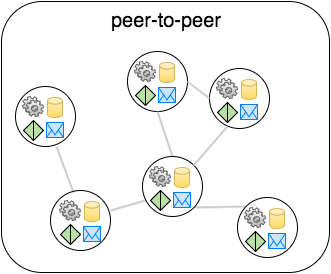
\includegraphics[width=\textwidth]{res/fig/scafi-p2p.png}
    %     \caption{Architettura \emph{peer-to-peer}}%
    %     \label{fig:scafi:p2p}
    %   \end{subfigure}
    %   \hspace{0.15\textwidth} % a differenza di \hfill il commento serve per non aggiungere spazi
    %   \begin{subfigure}{0.35\textwidth}
    %     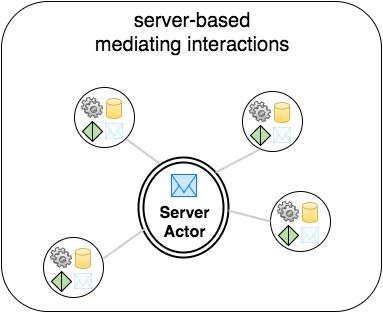
\includegraphics[width=\textwidth]{res/fig/scafi-server-based.png}
    %     \caption{Architettura \emph{server-based}}%
    %     \label{fig:scafi:server-based}
    %   \end{subfigure}
    %   \caption[
    %     Architetture della piattaforma distribuita di ScaFi
    %   ]{
    %     Architetture della piattaforma distribuita di ScaFi.

    %     Figura ripresa da~\cite{AggregatecomputingVlsubicomp16}.
    %   }%
    %   \label{fig:scafi}
    % \end{figure}

    Nel caso centralizzato, è la piattaforma a mantenere le posizioni spaziali dei dispositivi e a gestire il vicinato, secondo il modello tradizionale client-server.
\end{description}

Dato che si appoggia su Scala come linguaggio ospite, è in grado di interoperare con Java e gli altri linguaggi in grado si eseguire in ambiente JVM, mantenendo il solido \emph{type-system} messo a disposizione da Scala e i suoi costrutti funzionali.
